\documentclass{article}
\usepackage[utf8]{inputenc}
\usepackage{lmodern,textcomp}

\usepackage{graphicx}
\graphicspath{ {./} }

%Paquets codi maco
\usepackage{listings}
\usepackage{textcomp}
\usepackage{xcolor}
\definecolor{listinggray}{gray}{0.9}
\definecolor{lbcolor}{rgb}{0.9,0.9,0.9}

\lstdefinestyle{JavaStyle}{
        backgroundcolor=\color{lbcolor},
    tabsize=4,
    language=Python,      % choose the language of the code
        basicstyle=\scriptsize,     % the size of the fonts that are used for the code
        upquote=true,
        aboveskip={1.5\baselineskip},
        columns=fixed,
        showstringspaces=false,
        extendedchars=false,
        breaklines=true,
        prebreak = \raisebox{0ex}[0ex][0ex]{\ensuremath{\hookleftarrow}},
        frame=single,
        numbers=left,
        showtabs=false,
        showspaces=false,
        showstringspaces=false,
        identifierstyle=\ttfamily,
        keywordstyle=\color[rgb]{0,0,1},
        commentstyle=\color[rgb]{0.026,0.112,0.095},
        commentstyle=\itshape\color{green!40!black},
        stringstyle=\itshape\color{red!90!black},
        numberstyle=\itshape\color{yellow!50!black}
}




\title{Memòria}
\author{Albert Acebrón}
\date{Febrer 2019}

\begin{document}

\maketitle

\section*{Preguntes 1 i 2}

%1. Se suposa que el canvi d’horari entre estiu i hivern comportava un estalvi d’energia. És realment així? Perquè?

Per resoldre aquesta qüestió aproximarem, mitjançant simulacions, l’energia utilitzada per una població durant tot l’any utilitzant els dos tipus d’horari, és a dir, aproximant el consum anual d’energia d’una població que no canvii d’hora i el d’una població que segueixi els canvis d’hora entre estiu i hivern.

Per fer aquestes aproximacions realitzarem diverses assumpcions:
\begin{itemize}
    \item L’hora en que els individus d’una població es desperten vista com a variable aleatòria obeeix una distribució normal amb mitja de 420.39 minuts respecte 0:00\footnotemark[\ref{sleepstats}] i desviació estàndard de 40.7 minuts\footnote{\label{sleepstats}https://www.ncbi.nlm.nih.gov/pmc/articles/PMC2818595/}.
    \item L’interval de temps en que un membre de la població està al llit es regeix per una distribució normal amb mitja 461.4 minuts\footnotemark[\ref{sleepstats}] i desviació estàndard de 72.1 minuts\footnotemark[\ref{sleepstats}].
    \item Amb un nombre de mostres de 1.000 l’aproximació obtinguda és suficient\footnote{\label{aproxSuficient}Diem que una aproximació és suficient quan aquesta aproximació convergeix cap a un valor i la diferència entre el resultat obtingut per aquesta aproximació i una altra amb més precisió és negligible, és a dir, que utilitzar més precisió canvia el resultat molt poc.}.
    \item Estimant el consum d’energia en intervals d’una hora obtenim una aproximació suficient\footnotemark[\ref{aproxSuficient}].
    \item La funció que calcula la radiació del Sol és la descrita a l'Àpendix II.
    \item Durant el temps en que està despert, un individu utilitza una font de llum que es pot modelitzar amb una bombeta de 20 Watts\footnote{https://ca.wikipedia.org/wiki/Bombeta\_el\%C3\%A8ctrica} i una font de calor (ex: calefacció) que consumeix $\frac{1639}{20}=81.95$ Watts per metre quadrat\footnote{https://www.caloryfrio.com/calefaccion/calefaccion-instalaciones-componentes/calcular-la-potencia-calorifica-para-una-casa-o-habitacion.html}, és a dir, té un consum d'energia de 101.95 Watts.
\end{itemize}

Executant les simulacions utilitzant el codi proporcionat a l'apèndix I obtenim el següent resultat per la latitud de Barcelona:
\begin{itemize}
    \item Energia sense canvi d'hora: 731552775.4536844 J
    \item Energia amb canvi d'hora: 674009242.0969346 J
    \item Diferència: 57543533.3567498 J = 15.98431482131938886 kWh
\end{itemize}

Així doncs, com que a Catalunya hi ha 7.543.825 habitants\footnote{https://www.idescat.cat/pub/?id=aec\&n=245} implementar el canvi d'horari implica un estalvi energètic de 120582873.756939739 kWh, que representa un 0.079811721\% de l'energia total utilitzada a Catalunya anualment, ja que el consum d'energia total a Catalunya és de 12.990,9 ktep = 151084167000 kWh d'acord amb l'Institut Català d'Energia\footnote{http://icaen.gencat.cat/ca/energia/estadistiques/resultats/anuals/balanc\_energetic/}, una conclusió que s'alinea amb els resultats obtinguts en recerca prèvia\footnote{https://doi.org/10.1016/j.enpol.2007.05.021}.

%2. De quines quantitats d’energia estaríem parlant? I en termes econòmics? Depèn de la latitud?

Donat que la diferència en consum d'energia entre la simulació sense canvi d'hora i la de amb canvi d'hora és de 120582873.756939739 i actualment el preu de la energia elèctrica és de 0.23 €/kWh\footnote{https://en.wikipedia.org/wiki/Electricity\_pricing}, llavors el estalvi econòmic causat per la implementació del canvi d'horari és de $120582873.756939739\cdot 0.23=27734060.96409614$€.

Està clar que l'estalvi energètic dependrà de la latitud, ja que la funció de la radiació solar depèn directament de la latitud, però la pregunta és: com de forta és aquesta dependència?
Simulant l'estalvi d'energia de poblacions a diverses latituds i visualitzant els resultats obtenim el següent gràfic, en el que es pot apreciar la correlació entre latitud (en graus des de l'equador) i estalvi d'energia (en Joules/persona*any):

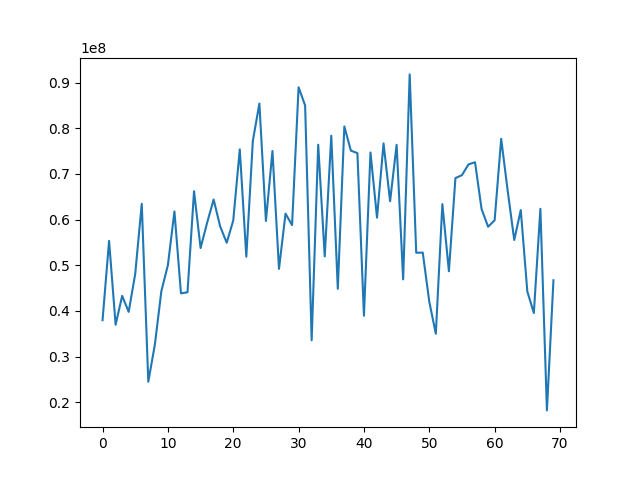
\includegraphics[scale=0.8]{Figure_1.png}
Donat que tenim que executar moltes simulacions (2 per cada latitud) per tal de fer el gràfic, he agafat un nombre de mostres petit (100). Veient el gràfic, sembla bastant possible que aquest nombre de mostres sigui massa petit i això faci que la naturalesa probabilística de les simulacions es faci més visible i els resultats siguin més variables. Això es podria resoldre executant simulacions amb un nombre de mostres més elevat però per falta de temps i recursos em resulta impossible.

\section*{Pregunta 3}
%3. Hi ha altres factors a tenir en compte a banda del possible estalvi energètic?

D'acord amb diversos estudis\footnote{http://www.europarl.europa.eu/thinktank/en/document.html?reference=EPRS\_STU\%282017\%29611006}\footnote{https://ec.europa.eu/transport/sites/transport/files/facts-fundings/studies/doc/2014-09-19-the-application-of-summertime-in-europe.pdf}\footnote{\label{eu-consultation}https://ec.europa.eu/info/consultations/2018-summertime-arrangements\_en} realitzats per grups de recerca i comissions de la Unió Europea, a part del sector de l'energia el canvi d'horari afecta els següents sectors/camps:
\begin{itemize}
    \item Mercats/Economia: Hi ha suficient evidencia com per concloure que diferencies en la implementació del canvi d'horaris entre països veïns portarien a un augment dels costos en les industries del comerç, transport, turisme i comunicacions, disminuint la eficiència dels mercats.
    \item Salut: S'estima que el canvi d'horari genera efectes positius sobre la salut a causa d'un increment en activitats a l'aire lliure. No obstant, recerca en el camp de la chronobiologia suggereix que el impacte en la salut d'alterar el bioritme humà a causa dels canvis d'horari també és important. No hi suficient evidencia per concloure si en general els efectes positius sobrepassen els negatius o és al revés.
    \item Seguretat Viària: No hi ha evidencia conclusiva que relacioni els canvis d'horari amb accidents de tràfic però podria ser possible que els canvis d'horari augmentessin el nombre d'accidents durant uns dies a causa de la falta de son o que l'extensió de hores amb sol durant l'estiu portés a una disminució dels accidents. Encara que s'observa que hi ha una correlació entre accidents de tràfic i canvis d'horari no s'ha pogut determinar si hi ha una relació de causalitat o simplement correlació.
    \item Agricultura: Anteriorment hi podia haver un empitjorament de la producció causat per canvis en el bioritme dels animals (ja que els canvis d'horari es traslladaven a canvis en l'horari de les granges) però com actualment la gran majoria de granges utilitzen tecnologia automatitzada aquest ha deixat de ser un problema. Podria ser el cas que augmentar les hores de sol a l'estiu permetis treballar més hores en activitats agrícoles com la collita. 
\end{itemize}

Com que el canvi d'horari afecta tots aquests camps a part del sector de la energia, es tindrien que tenir en compte a l'hora de prendre qualsevol decisió que involucrés canvis d'horari.

\section*{Pregunta 4}
%4. Quina seria la decisió més adequada per a Catalunya? (Si manté l’horari d’estiu o bé el d’hivern i en quin fus horari s’integra)

D'acord amb l'informe realitzat per la comunitat europea\footnotemark[\ref{eu-consultation}] sobre el canvi horari, la millor decisió per Catalunya és simplement copiar l'horari que implementin els països veïns a Catalunya, ja que la diferència en costos energètics que pot suposar utilitzar un horari a un altre són negligibles comparats amb els alts costos que apareixerien en el comerç entre països i les dificultats afegides en les àrees de transport, comunicacions i viatges transfronterers.

En cas de que els països veïns seguissin l'horari de Catalunya o poguéssim ignorar els altres països, trobarem l'horari òptim fent simulacions del consum d'energia en els diferents horaris:
\begin{itemize}
    \item Horari d'hivern a GMT+0: 866040378.3897454 J/persona*any
    \item Horari d'estiu a GMT+0 o horari d'hivern a GMT+1: 731552775.4536844 J/persona*any
    \item Horari d'estiu a GMT+1: 666986692.3970932 J/persona*any
\end{itemize}

Podem veure que el consum d'energia mínim es dóna quan Catalunya es troba al fus horari GMT+1 i segueix l'horari d'estiu.


\section*{Apèndix I: Codi utilitzat en la simulació}

\begin{lstlisting}[style=JavaStyle]
import numpy as np

def cos(angle):
    return np.cos(np.deg2rad(angle))

def sin(angle):
    return np.sin(np.deg2rad(angle))

def arcsin(val):
    return np.degrees(np.arcsin(val))

def solarRadiation(timeOfDay, day, latitude):
    declination=arcsin(sin(-23.44) * cos((360/365.24)*(day+10)+(360/np.pi)* 0.0167 * sin((360/365.24)*(day-2))))
    radiation=1367*0.53*(sin(declination)*sin(latitude)+cos(declination)*cos(latitude)*cos(((timeOfDay-12*60)/(24*60))*360))
    return radiation if radiation>=0 else 0
\end{lstlisting}
radiation.py

\begin{lstlisting}[style=JavaStyle]
import numpy as np
from radiation import solarRadiation

#Params
MINIMUM_LIGHT=101.95 #in Watts


def simulate(LATITUDE, DAYLIGHT_SAVINGS, SAMPLES):
    #LATITUDE in degrees from equator
    #DAYLIGHT_SAVINGS=False|True -> Simulació amb canvi d'horari?
    wakingTime=np.random.normal(420.39, 40.7, SAMPLES) #in minutes
    awakeHours=np.random.normal(24*60-461.4, 72.1, SAMPLES) #in minutes
    energy=0
    for i in range(SAMPLES): #Loop over samples
        for d in range(365): #Loop over days in year
            for hour in range(24):
                m=hour*60
                if m>wakingTime[i] and m<wakingTime[i]+awakeHours[i]: #Awake?
                    radiation=solarRadiation((m - (60 if (DAYLIGHT_SAVINGS and d>90 and d<300) else 0))%(24*60), d+(1 if (m>(24*60)) else 0), LATITUDE)
                    if radiation<MINIMUM_LIGHT: #Enough light?
                        energy+=(MINIMUM_LIGHT-radiation)*60*60
        print("sample %d done"%i)

    energy=energy/SAMPLES
    return energy

if __name__ == "__main__":
    print(simulate(41.3818, False, 1000)) #Latitud de Barcelona
\end{lstlisting}
simulation.py

\section*{Apèndix II: Funció de la radiació del sol}
La radiació màxima del sol que arriba a la terra, també coneguda com a constant solar\footnote{\label{sunstuff}https://www.researchgate.net/profile/Mohamad\_Kharseh/post/What\_is\_the\_extra-terrestrial\_solar\_radiance\_F0/attachment/59d63e0ac49f478072ea8d7b/AS\%3A273765705945088\%401442282238044/download/Solar+Radiation+Calculation.pdf}, és $1367 W/m^2$. D'aquesta radiació només un 53\% arriba a la superfície de la terra\footnotemark[\ref{sunstuff}] a causa de la refracció i absorció de radiació per l'atmosfera, i la radiació sol ser menor encara perquè depèn del angle en que la llum incideix sobre la terra, que ve donat per\footnote{http://rammb.cira.colostate.edu/wmovl/vrl/tutorials/euromet/courses/english/nwp/n5720/n5720005.htm}:
$$\cos(\theta)=\sin(\delta)\sin(\phi)+\cos(\delta)\cos(\phi)\cos(\omega)$$
on $\phi$ és la latitud en graus, $\omega$ és l'angle d'hora local\footnote{https://en.wikipedia.org/wiki/Hour\_angle}, que és $\frac{hora-12}{24}360$, i $\delta$ és la declinació del sol, que ve donada per\footnote{https://en.wikipedia.org/wiki/Position\_of\_the\_Sun\#Declination\_of\_the\_Sun\_as\_seen\_from\_Earth}:
$$\delta=\arcsin \left[\sin \left(-23.44^{\circ }\right)\cdot \cos \left({\frac {360^{\circ }}{365.24}}\left(N+10\right)+{\frac {360^{\circ }}{\pi }}\cdot 0.0167\sin \left({\frac {360^{\circ }}{365.24}}\left(N-2\right)\right)\right)\right]$$
on $N$ és el dia de l'any. Així doncs, la radiació solar sol és de $1367\cdot0.53\cdot\cos(\theta)$ Watts per metre quadrat.
\end{document}

